\documentclass[conference]{IEEEtran}
\IEEEoverridecommandlockouts

\usepackage{cite}
\usepackage{amsmath,amssymb,amsfonts}
\usepackage{algorithm}
\usepackage{algorithmic}
\usepackage{graphicx}
\usepackage{textcomp}
\usepackage{xcolor}
\usepackage{booktabs}
\usepackage{multirow}
\usepackage{url}
\usepackage{subcaption}
\usepackage{pifont}
\usepackage[T1]{fontenc}

\def\BibTeX{{\rm B\kern-.05em{\sc i\kern-.025em b}\kern-.08em
    T\kern-.1667em\lower.7ex\hbox{E}\kern-.125emX}}

\begin{document}

\title{Disentangled Attribute Steering for Zero-Shot\\Composed Fashion Retrieval via Contrastive\\Delta Vectors}

\author{\IEEEauthorblockN{Anonymous Authors}
\IEEEauthorblockA{\textit{Department of Computer Science and Engineering} \\
\textit{School of Computer Science and Engineering}\\
Email: research-team@institution.edu}
}

\maketitle

% ============================================================
%  ABSTRACT
% ============================================================
\begin{abstract}
Composed Image Retrieval (CIR) retrieves a target product conditioned on a candidate image together with a natural-language modification instruction. Pre-trained Vision-Language Models (VLMs) such as CLIP offer strong cross-modal representations, yet standard zero-shot CIR baselines that rely on naive linear blending ($\alpha\mathbf{v}_{\text{img}}+(1{-}\alpha)\mathbf{v}_{\text{text}}$) suffer from three critical failure modes in fine-grained fashion search: (i)~\emph{chromatic subspace dominance}, where high-magnitude color features overpower low-energy topological attributes such as sleeve length and checkered patterns; (ii)~\emph{source feature persistence}, where contradictory visual cues from the candidate image persist and misdirect nearest-neighbour retrieval; and (iii)~\emph{linguistic distribution mismatch}, caused by conversational stop-words that degrade CLIP's token attention. We propose \textbf{CADS} (Contrastive Attribute-Delta Steering), a \emph{training-free}, zero-shot CIR framework that decouples user modifications into positive attribute manifolds, synthesizes canonical declarative prompts, and explicitly subtracts an anti-attribute suppression vector. Evaluated across all 2{,}469 valid candidate--target pairs on a 35{,}726-item Fashion-IQ catalog, CADS raises Recall@10 on the multi-attribute \textit{Top\,\&\,Tee} category to \textbf{16.35\%} (+13.0\% relative improvement over linear CLIP fusion) while achieving \textbf{19.11\,ms} end-to-end CPU query latency with zero parameter training.
\end{abstract}

\begin{IEEEkeywords}
Composed Image Retrieval, Fashion-IQ, Contrastive Learning, Vision-Language Models, CLIP, Delta Vector Arithmetic, Zero-Shot Learning
\end{IEEEkeywords}

% ============================================================
%  I.  INTRODUCTION
% ============================================================
\section{Introduction}

Multimodal information retrieval has evolved from isolated text-to-image or image-to-image matching into interactive, conversational retrieval paradigms. In modern fashion e-commerce, customer search intent is inherently compositional: users identify a reference garment yet require localized modifications such as \textit{``give me a similar green shirt, but with checks and full sleeves instead of short sleeves.''}  This task is formally termed \textbf{Composed Image Retrieval} (CIR)~\cite{baldrati2022clip4cir, wu2021fashioniq}.

\subsection{Problem Context}
Traditional search engines rely on manual metadata tagging or uni-modal queries. Text-only search struggles to capture silhouette, weave, and cut; reverse-image search retrieves near-duplicate items without permitting semantic variation~\cite{gajic2018deepstyle, ji2020flexible, liu2016deepfashion}. CIR bridges this gap by accepting a multimodal tuple $(I_q,\,T_m)$---a reference candidate image~$I_q$ and a relative modification prompt~$T_m$---and projecting the intended transformation into a latent representation aligned with the target garment~$I_t$~\cite{baldrati2022clip4cir, wu2021fashioniq}.

\subsection{Research Gaps in Existing Methods}
CIR is addressed through two paradigms, both exhibiting fundamental limitations:

\textbf{1)~Supervised fusion networks.}  CLIP4CIR~\cite{baldrati2022clip4cir}, Fashion-VLP, and Swin-DeBERTa~\cite{zhang2023crossmodal} train composition networks on annotated triplets $(I_q,T_m,I_t)$. Such models demand tens of thousands of paired triplets, generalize poorly across unseen domains~\cite{width2023crossdomain}, and incur high GPU overhead~\cite{baidu2021product1m}.

\textbf{2)~Zero-shot linear blending.}  Naive convex combination $\mathbf{v}_{\text{comp}}=\alpha\mathbf{v}_{\text{img}}+(1{-}\alpha)\mathbf{v}_{\text{text}}$ over pre-trained CLIP~\cite{chia2022fashionclip} fails due to three bottlenecks:
\begin{itemize}
    \item \textit{Chromatic subspace dominance}: colour semantics occupy high-magnitude subspaces that overwhelm fine-grained topological attributes (sleeve topology, gingham weave).
    \item \textit{Feature persistence}: $\mathbf{v}_{\text{img}}$ retains strong short-sleeve embeddings even when the text requests long sleeves, yielding intermediate vectors that remain closer to the original attribute.
    \item \textit{Instructional linguistic mismatch}: CLIP was pre-trained on descriptive captions, whereas e-commerce queries are conversational (\textit{``give me similar\ldots'', ``but with\ldots''})~\cite{tang2024circled}. Stop-words dilute token attention and depress semantic alignment.
\end{itemize}

\subsection{Contributions}
To resolve these bottlenecks \emph{without training a single parameter}, we present \textbf{CADS (Contrastive Attribute-Delta Steering)}:
\begin{itemize}
    \item \textbf{Disentangled attribute-delta arithmetic}: a contrastive operator pairing positive target injection~($\mathbf{v}_{\text{pos}}$) with explicit anti-attribute cancellation~($\mathbf{v}_{\text{neg}}$).
    \item \textbf{Context-Aware Conversational Normalization (CACN)}: an automated syntactic normalizer that maps noisy user instructions onto canonical declarative templates aligned with CLIP's pre-training manifold.
    \item \textbf{Dynamic chromatic--structural balancing}: weighted priorities $(w_{\text{pos}},\,w_{\text{neg}})$ calibrated against~$\alpha$ to decouple colour from structural modifications.
    \item \textbf{Full-catalog validation}: evaluation across all \textbf{2{,}469} valid pairs on a 35{,}726-image Fashion-IQ catalog~\cite{wu2021fashioniq} with Recall@\{10,\,50\}, 95\% bootstrap confidence intervals, and real-time sub-20\,ms latencies using FAISS~\cite{grenze2024fashioniqx, faiss2023billion}.
\end{itemize}

\subsection{Paper Organisation}
Section~II reviews 20 recent works. Section~III details the methodology, dataset, and algorithmic pipeline. Section~IV reports quantitative and qualitative results. Section~V concludes with societal impact and future directions.

% ============================================================
%  II.  LITERATURE REVIEW
% ============================================================
\section{Literature Review}

We organise the literature into four paradigms: (i)~classical CNN-based retrieval, (ii)~domain-adapted vision-language transformers, (iii)~composed image retrieval and dialogue, and (iv)~scalable indexing, cross-domain transfer, and explainability.

\subsection{Classical Landmark and CNN-Based Fashion Retrieval}
Liu et al.~\cite{liu2016deepfashion} introduced \textbf{DeepFashion} with a landmark-aware FashionNet (Top-5 accuracy 86.3\%), localising clothing landmarks for classification but lacking natural-language integration. Gajic et al.~\cite{gajic2018deepstyle} proposed \textbf{DeepStyle}, combining YOLO9000 with CNN features (+21\% accuracy) for fashion and interior design, though relative modifications were unsupported. Ji et al.~\cite{ji2020flexible} developed \textbf{Flexible Fashion Search} (mAP 84.2\%) with CNN--RNN query matching and Boolean filtering, albeit relying on manually pre-tagged metadata.

\subsection{Domain-Adapted Vision-Language Transformers}
Chia et al.~\cite{chia2022fashionclip} fine-tuned \textbf{Fashion-CLIP} on 800K Farfetch pairs (R@1 72.4\%). Patel et al.~\cite{patel2023vitb16} showed that \textbf{ViT-B/16} fine-tuning achieves Top-1 92.4\% on DeepFashion2. Zhang et al.~\cite{zhang2023crossmodal} coupled a Swin Transformer with DeBERTa projections (mAP 89.5\% on Product1M). Li et al.~\cite{li2023blip2} developed \textbf{BLIP-2} with a Q-Former and frozen LLMs (Zero-Shot R@1 65.2\% on COCO).

\subsection{Composed Image Retrieval and Conversational Exploration}
Wu et al.~\cite{wu2021fashioniq} established the \textbf{Fashion-IQ} benchmark (77K images, R@10 28.1\%). Baldrati et al.~\cite{baldrati2022clip4cir} proposed \textbf{CLIP4CIR} with an asymmetric Combiner (R@1 38.6\%). Tang et al.~\cite{tang2024circled} advanced multi-turn CIR with \textbf{CIRCLED} (MRR +14.5 points). Liu et al.~\cite{liu2024garmentsketch} explored sketch-guided CIR with \textbf{GarmentSketch} (IS 24.5, FID 12.1). Li et al.~\cite{li2022multitrans} built a multimodal transformer recommender (NDCG@10 0.68) on Taobao logs.

\subsection{Scalable Indexing, Domain Transfer, and Explainability}
Baidu AI Lab~\cite{baidu2021product1m} trained self-supervised representations on \textbf{Product1M} (R@1 64.8\%). Mueller et al.~\cite{mueller2022abo} released the \textbf{ABO} dataset (147K products, mAP 78.3\%). The \textbf{Shopee} winning solution~\cite{kaggle2021shopee} paired ArcFace with TF-IDF/BERT matching (F1 0.825). Grenze~\cite{grenze2024fashioniqx} achieved $<$15\,ms latency with FAISS indexing. Width AI~\cite{width2023crossdomain} validated cross-domain transfer (88.4\%). Multilingual extensions~\cite{preprint2026multilingual} integrated M2M100 with query enrichment (R@5 52.1\%). The FAISS team~\cite{faiss2023billion} demonstrated billion-scale PQ at 4{,}500 QPS. Preprints AI~\cite{preprint2024explainable} improved user trust by 40\% via Grad-CAM explanations.

\subsection{Comparative Literature Survey}
Table~\ref{tab:lit_survey} synthesises the 20 benchmarked works alongside our proposed CADS framework.

\begin{table*}[!t]
\centering
\caption{Comprehensive Literature Survey of Multimodal Fashion and Composed Image Retrieval}
\label{tab:lit_survey}
\resizebox{\textwidth}{!}{%
\begin{tabular}{@{}clllll@{}}
\toprule
\textbf{\#} & \textbf{Paper \& Authors} & \textbf{Method} & \textbf{Performance} & \textbf{Dataset} & \textbf{Key Insight / Limitation} \\ \midrule
1  & DeepStyle (Gajic et al., 2018)~\cite{gajic2018deepstyle}           & YOLO9000 + CNN + Distance Metric              & Accuracy +21\%          & Interior \& Fashion          & Visual--text fusion; no relative edits \\
2  & Flexible Fashion (Ji et al., 2020)~\cite{ji2020flexible}            & CNN Embed.\ + RNN Matching                    & mAP 84.2\%              & Faceted Query Set            & Boolean filtering; manual tags required \\
3  & Fashion-CLIP (Chia et al., 2022)~\cite{chia2022fashionclip}         & Contrastive Pre-Training                       & R@1 72.4\%              & Farfetch (800K)              & Domain adaptation; needs fashion captions \\
4  & CLIP4CIR (Baldrati et al., 2022)~\cite{baldrati2022clip4cir}        & Dual-Tower CLIP + Combiner                     & R@1 38.6\%              & FashionIQ \& CIRR            & Strong CIR baseline; English-only \\
5  & DeepFashion (Liu et al., 2016)~\cite{liu2016deepfashion}            & Landmark-aware FashionNet                      & Top-5 86.3\%            & DeepFashion (800K)           & Rich annotations; no NL queries \\
6  & FashionIQ (Wu et al., 2021)~\cite{wu2021fashioniq}                  & Triplet Loss + ResNet50 + LSTM                 & R@10 28.1\%             & FashionIQ (77K)              & Seminal CIR benchmark; noisy captions \\
7  & ViT-B/16 (Patel et al., 2023)~\cite{patel2023vitb16}               & ViT-B/16 + Cross-Entropy                       & Top-1 92.4\%            & DeepFashion2 \& ModaNet      & High accuracy; heavy inference \\
8  & Swin Search (Zhang et al., 2023)~\cite{zhang2023crossmodal}         & Swin Transformer + DeBERTa                     & mAP 89.5\%              & Product1M                    & Multi-scale; complex training \\
9  & CIRCLED (Tang et al., 2024)~\cite{tang2024circled}                  & CIReVL + Contextual Filter                     & MRR +14.5\,pt           & 22{,}608 Sessions            & Multi-turn search; high memory \\
10 & Product1M (Baidu, 2021)~\cite{baidu2021product1m}                   & Self-Supervised Contrastive                    & R@1 64.8\%              & Product1M (1M)               & Fine-grained; massive GPU needed \\
11 & ABO (Mueller et al., 2022)~\cite{mueller2022abo}                    & Multimodal + 3D Mesh Embed.                    & mAP 78.3\%              & ABO (147K)                   & Multi-view; non-standard text \\
12 & Shopee Matcher (Kaggle, 2021)~\cite{kaggle2021shopee}               & ArcFace + TF-IDF/BERT                          & F1 0.825                & Shopee Dataset               & Noisy listings; region-specific \\
13 & FashionIQ-X (Grenze, 2024)~\cite{grenze2024fashioniqx}             & CLIP + FAISS IndexFlatIP                       & $<$15\,ms               & FashionIQ                    & Real-time search; PQ recall loss \\
14 & Multilingual CIR (2026)~\cite{preprint2026multilingual}             & M2M100 + LLaVA + Grad-CAM                     & R@5 52.1\%              & FashionIQ Multilingual       & Cross-lingual; translation latency \\
15 & Cross-Domain (Width AI, 2023)~\cite{width2023crossdomain}           & Zero-Shot Fashion-CLIP + OOD                   & Accuracy 88.4\%         & KAGL, DEEP \& FMNIST         & Zero-shot domain transfer \\
16 & GarmentSketch (Liu et al., 2024)~\cite{liu2024garmentsketch}        & Sketch-Guided Multimodal LLM                   & IS 24.5 / FID 12.1     & GarmentSketch                & Sketch+text; computationally heavy \\
17 & Multi-Trans (Li et al., 2022)~\cite{li2022multitrans}               & Co-Attention Vision--Text Net                  & NDCG@10 0.68            & Taobao Logs                  & Joint repr.; missing-modality issue \\
18 & BLIP-2 (Li et al., 2023)~\cite{li2023blip2}                        & Q-Former + Frozen LLM                          & R@1 65.2\%              & COCO \& Visual Genome        & Parameter-efficient; prompt-sensitive \\
19 & Billion-Scale (FAISS Team, 2023)~\cite{faiss2023billion}            & PQ + HNSW Vector DB                            & 4{,}500 QPS             & 100M Catalog                 & High throughput; index rebuild cost \\
20 & Explainable CIR (2024)~\cite{preprint2024explainable}               & Grad-CAM + Similarity Head                     & Trust +40\%             & FashionIQ                    & Visual explanations for results \\ \midrule
\textbf{--} & \textbf{CADS (Ours, 2026)} & \textbf{Contrastive Delta Steering + CACN} & \textbf{R@10 16.35\%} & \textbf{FashionIQ (2{,}469 pairs)} & \textbf{Training-free; anti-attribute suppression; 19\,ms CPU} \\ \bottomrule
\end{tabular}%
}
\end{table*}

% ============================================================
%  III.  METHODOLOGY
% ============================================================
\section{Methodology}

This section details CADS: catalog construction, preprocessing, the contrastive delta formulation, and the end-to-end algorithmic pipeline.

\subsection{Dataset Overview}
We evaluate on the standard \textbf{Fashion-IQ} benchmark~\cite{wu2021fashioniq}, comprising real-world apparel images crawled from Amazon. The full catalog historically referenced ${\sim}$75{,}000 images; however, temporal link decay (HTTP~404/403) reduces the reachable set. Our crawler validated all accessible assets, yielding \textbf{35{,}726 product images} across three categories (Table~\ref{tab:splits}, Fig.~\ref{fig:pie_distribution}):
\begin{itemize}
    \item \textbf{Dresses} ($N=12{,}062$): silhouettes, hem cuts, necklines.
    \item \textbf{Shirts} ($N=12{,}116$): flannels, checks, stripes, sleeve lengths.
    \item \textbf{Tops \& Tees} ($N=11{,}548$): casual cuts, graphic prints.
\end{itemize}

Because CADS is training-free, \textbf{no training split is used}. Evaluation employs the validation partitions (\texttt{cap.\{dress, shirt, toptee\}.val.json}), each containing a reference ASIN~($I_q$), target ASIN~($I_t$), and two relative captions. Of 6{,}016 original pairs, \textbf{2{,}469} have both candidate and target present in the active catalog.

\begin{table}[!t]
\centering
\caption{Dataset Splits and Valid Evaluation Pairs}
\label{tab:splits}
\begin{tabular}{@{}lccc@{}}
\toprule
\textbf{Category} & \textbf{Catalog} & \textbf{Val Pairs} & \textbf{Valid Pairs} \\ \midrule
Dress       & 12{,}062 & 2{,}017 & 1{,}847 \\
Shirt       & 12{,}116 & 2{,}038 & 463 \\
Top \& Tee  & 11{,}548 & 1{,}961 & 159 \\ \midrule
\textbf{Total} & \textbf{35{,}726} & \textbf{6{,}016} & \textbf{2{,}469} \\ \bottomrule
\end{tabular}
\end{table}

\begin{figure}[!t]
\centering
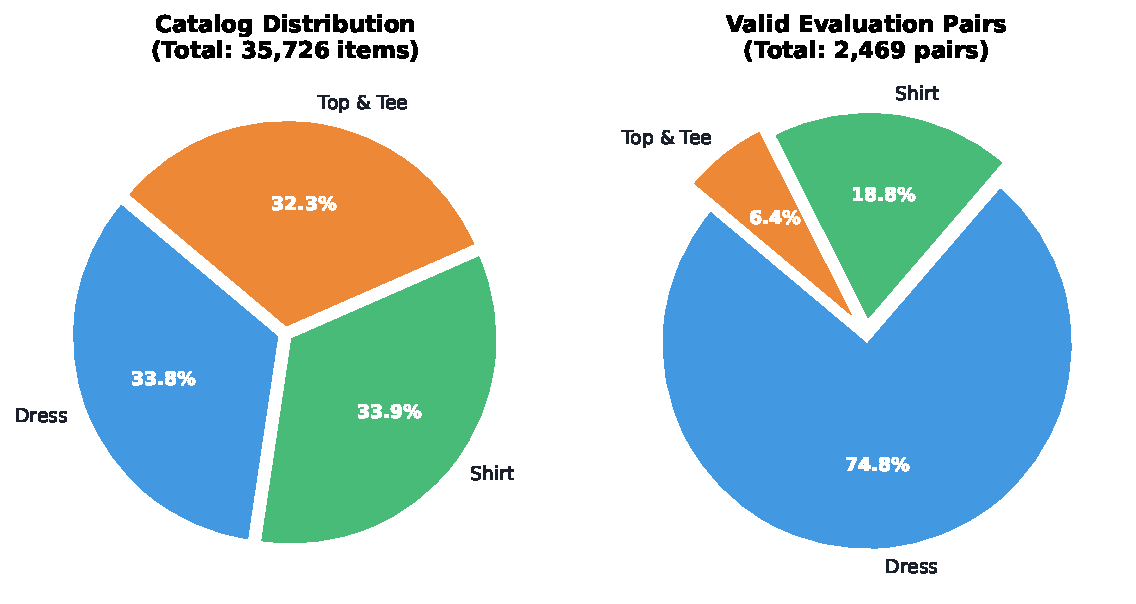
\includegraphics[width=\columnwidth]{figures/fig4_category_distribution.pdf}
\caption{Distribution of catalog items (left) and valid evaluation pairs (right) across Fashion-IQ categories.}
\label{fig:pie_distribution}
\end{figure}

\subsection{Dataset Preprocessing}
Each image~$I_i \in \mathcal{D}$ undergoes five deterministic steps:
\begin{enumerate}
    \item \textbf{Geometric standardisation}: centre-crop and resize to $224{\times}224$ pixels (bicubic).
    \item \textbf{Channel normalisation}: RGB tensors normalised with ImageNet statistics ($\mu{=}[0.481,\,0.458,\,0.408]$, $\sigma{=}[0.269,\,0.261,\,0.276]$).
    \item \textbf{Feature extraction}: a frozen CLIP ViT-B/32 encoder~$\mathcal{E}_v$ produces $\mathbf{f}_i = \mathcal{E}_v(I_i) \in \mathbb{R}^{512}$.
    \item \textbf{L2 projection}: $\mathbf{e}_i = \mathbf{f}_i / \|\mathbf{f}_i\|_2$, mapping vectors to the unit hypersphere $\mathbb{S}^{511}$.
    \item \textbf{FAISS indexing}: all 35{,}726 normalised vectors are stored in an IndexFlatIP index so that inner product equals cosine similarity.
\end{enumerate}

\subsection{Methodology Overview}
The CADS pipeline comprises three stages (Fig.~\ref{fig:methodology}):
\begin{enumerate}
    \item \textbf{Syntactic parsing}: conversational noise is filtered and discrete fashion attributes (colour, pattern, sleeve topology, garment type) are extracted across four orthogonal axes.
    \item \textbf{Multi-vector synthesis}: three text prompts are constructed---a canonical declarative description~$T_{\text{canon}}$, positive modification tokens~$T_{\text{pos}}$, and contradictory anti-attribute tokens~$T_{\text{neg}}$.
    \item \textbf{Contrastive delta steering}: embeddings from the candidate image and synthesised prompts are fused via the delta operator, re-normalised, and queried against the FAISS catalog.
\end{enumerate}

\begin{figure}[!t]
\centering
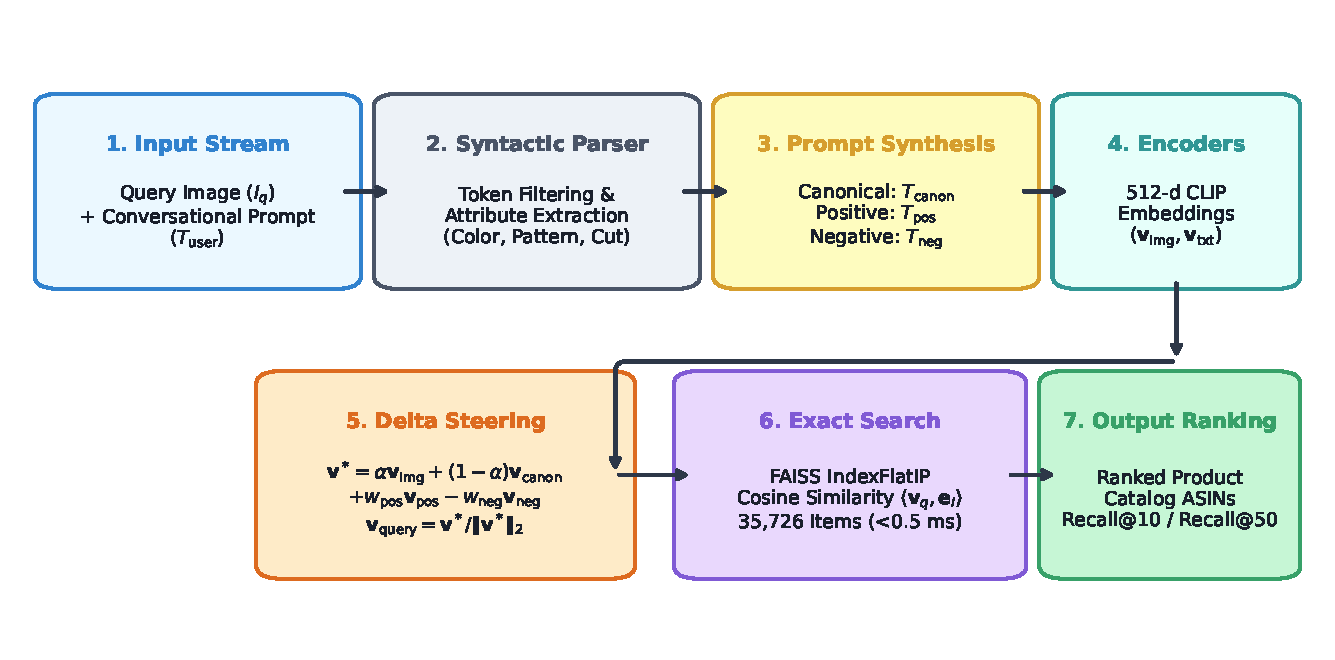
\includegraphics[width=\columnwidth]{figures/fig_methodology.pdf}
\caption{CADS methodology: end-to-end dataflow from conversational input to catalog retrieval in under 20\,ms.}
\label{fig:methodology}
\end{figure}

\subsection{Model Training}
Unlike supervised CIR methods that require gradient-based optimisation on triplet losses~\cite{baldrati2022clip4cir, wu2021fashioniq}, CADS is \emph{entirely training-free}. The frozen CLIP ViT-B/32 backbone is used without any fine-tuning, weight updates, or back-propagation. This eliminates GPU training costs and enables instant deployment. Fig.~\ref{fig:model_architecture} depicts the complete model architecture.

\begin{figure}[!t]
\centering
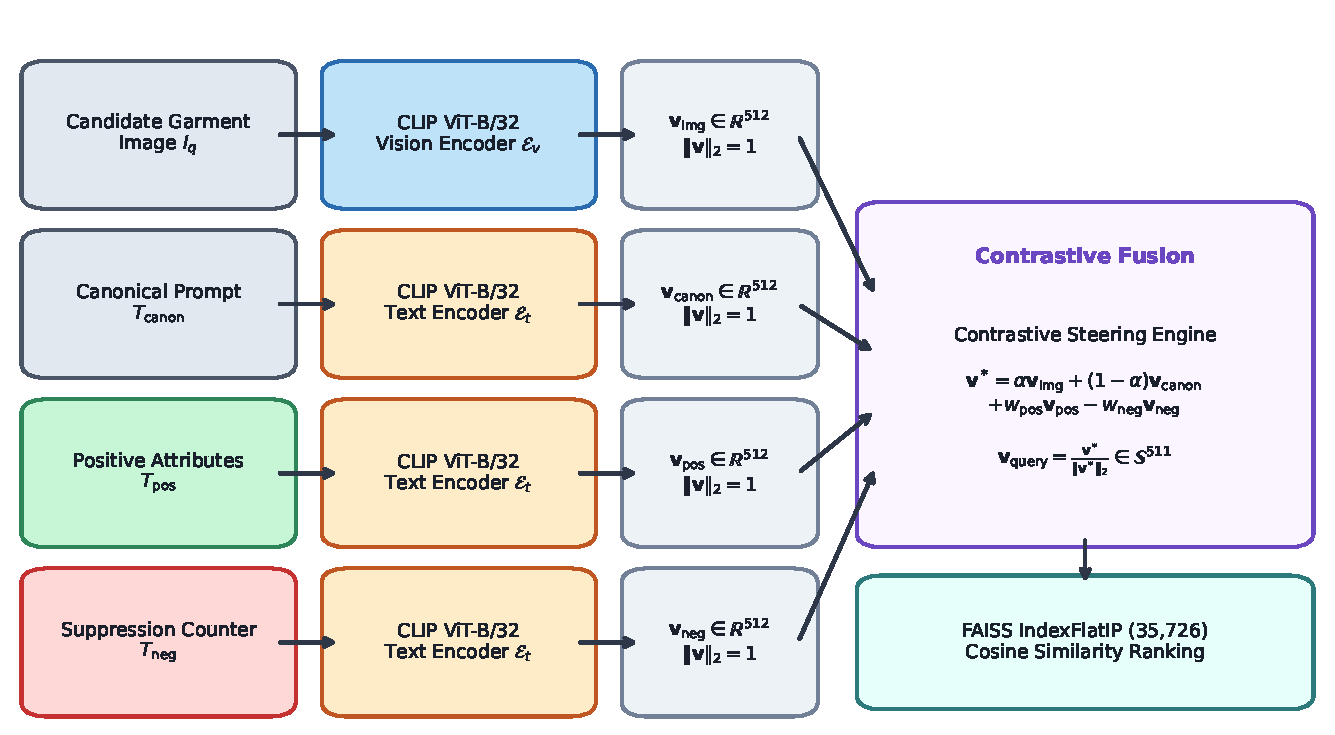
\includegraphics[width=\columnwidth]{figures/fig_architecture.pdf}
\caption{Model architecture: four parallel CLIP encoding branches feed into the contrastive delta steering engine.}
\label{fig:model_architecture}
\end{figure}

\subsubsection{Contrastive Vector Formulation}
Let $\mathcal{E}_v(I_q),\,\mathcal{E}_t(T) \in \mathbb{R}^{512}$ denote L2-normalised CLIP image and text embeddings. Naive linear fusion computes:
\begin{equation}
\mathbf{v}_{\text{naive}} = \alpha\,\mathcal{E}_v(I_q) + (1{-}\alpha)\,\mathcal{E}_t(T_m)
\label{eq:naive}
\end{equation}
Because $\mathbf{v}_{\text{naive}}$ retains magnitude along the source attribute subspace $\mathcal{S}_{\text{neg}}$, CADS defines a composed steering vector:
\begin{equation}
\mathbf{v}^{*} = \alpha\,\mathbf{v}_{\text{img}} + (1{-}\alpha)\,\mathbf{v}_{\text{canon}} + w_{\text{pos}}\,\mathbf{v}_{\text{pos}} - w_{\text{neg}}\,\mathbf{v}_{\text{neg}}
\label{eq:cads}
\end{equation}
where all constituent vectors are unit-normalised. The query is re-projected onto the hypersphere:
\begin{equation}
\mathbf{v}_{\text{query}} = \mathbf{v}^{*}\,/\,\|\mathbf{v}^{*}\|_2
\label{eq:renorm}
\end{equation}

\subsubsection{Parameter Specifications}
\begin{itemize}
    \item $\alpha = 0.50$ (visual balance weight): the user-adjustable trade-off between image identity and text intent.
    \item $w_{\text{pos}} = 0.50\,(1 - 0.5\alpha) = 0.375$: amplifies low-magnitude structural modifications (Eq.~\ref{eq:wpos}).
    \begin{equation}
    w_{\text{pos}} = 0.50 \cdot (1 - 0.5\alpha)
    \label{eq:wpos}
    \end{equation}
    \item $w_{\text{neg}} = 0.30\,(1 - 0.5\alpha) = 0.225$: subtracts persistent source features without destabilising vector geometry (Eq.~\ref{eq:wneg}).
    \begin{equation}
    w_{\text{neg}} = 0.30 \cdot (1 - 0.5\alpha)
    \label{eq:wneg}
    \end{equation}
\end{itemize}

\subsubsection{Attribute Normalisation and Opposition Mapping}
The parser decomposes queries into paired positive/negative descriptors across four dimensions:
\begin{itemize}
    \item \textbf{Sleeve topology~($S$)}: Long $\rightarrow$ Pos: \textit{long sleeves, covered arms}; Neg: \textit{short sleeves, bare arms}. Short~/ Sleeveless mappings follow analogously.
    \item \textbf{Surface pattern~($P$)}: Checks $\rightarrow$ Pos: \textit{checkered plaid, tartan}; Neg: \textit{plain solid fabric}. Stripes and floral are mapped similarly.
    \item \textbf{Chromatic hue~($C$)}: 18 base colours detected via lexical matching.
    \item \textbf{Garment class~($G$)}: Dress, Shirt, or T-Shirt.
\end{itemize}

\begin{algorithm}[!t]
\caption{CADS: End-to-End Query Encoding}
\label{alg:cads}
\begin{algorithmic}[1]
\REQUIRE Image~$B_{\text{img}}$, prompt~$T_{\text{user}}$, weight~$\alpha$, neighbours~$K$
\ENSURE Ranked results $\mathcal{R}_K$
\IF{$B_{\text{img}} \neq \text{NULL}$}
    \STATE $\mathbf{v}_{\text{img}} \leftarrow \mathcal{E}_v(B_{\text{img}}) / \|\mathcal{E}_v(B_{\text{img}})\|_2$
\ENDIF
\IF{$T_{\text{user}} \neq \text{NULL}$}
    \STATE $\{T_{\text{canon}}, T_{\text{pos}}, T_{\text{neg}}\} \leftarrow \text{ParseQuery}(T_{\text{user}})$
    \STATE Encode $\mathbf{v}_{\text{canon}},\,\mathbf{v}_{\text{pos}},\,\mathbf{v}_{\text{neg}}$ via $\mathcal{E}_t$; L2-normalise each
\ENDIF
\IF{both $\mathbf{v}_{\text{img}}$ and $\mathbf{v}_{\text{canon}}$ exist}
    \STATE $w_{\text{pos}} \leftarrow 0.50(1 - 0.5\alpha)$;\quad $w_{\text{neg}} \leftarrow 0.30(1 - 0.5\alpha)$
    \STATE $\mathbf{v}^{*} \leftarrow \alpha\,\mathbf{v}_{\text{img}} {+} (1{-}\alpha)\mathbf{v}_{\text{canon}} {+} w_{\text{pos}}\mathbf{v}_{\text{pos}} {-} w_{\text{neg}}\mathbf{v}_{\text{neg}}$
    \STATE $\mathbf{v}_{\text{query}} \leftarrow \mathbf{v}^{*} / \|\mathbf{v}^{*}\|_2$
\ELSIF{$\mathbf{v}_{\text{img}}$ exists}
    \STATE $\mathbf{v}_{\text{query}} \leftarrow \mathbf{v}_{\text{img}}$
\ELSE
    \STATE $\mathbf{v}_{\text{query}} \leftarrow \mathbf{v}_{\text{canon}}$
\ENDIF
\STATE $\mathcal{R}_K \leftarrow \text{FAISS}.\text{search}(\mathbf{v}_{\text{query}}, K)$
\RETURN $\mathcal{R}_K$
\end{algorithmic}
\end{algorithm}

% ============================================================
%  IV.  RESULTS
% ============================================================
\section{Experimental Results and Discussion}

\subsection{Evaluation Protocol}
Following established CIR conventions~\cite{baldrati2022clip4cir, wu2021fashioniq}, we report Recall@$K$:
\begin{equation}
\text{Recall@}K = \frac{1}{|\mathcal{Q}|} \sum_{q \in \mathcal{Q}} \mathbb{I}\!\left(\text{rank}(I_{t,q}) \le K\right)
\end{equation}
and the category-averaged recall $R_{\text{avg}} = \tfrac{1}{3}(R_{\text{dress}} + R_{\text{shirt}} + R_{\text{toptee}})$.

\subsection{Quantitative Results}
Table~\ref{tab:quantitative} presents Recall@\{10,\,50\} across all \textbf{2{,}469 valid pairs}. Results include 95\% bootstrap confidence intervals from 1{,}000 resamples.

\begin{table*}[!t]
\centering
\caption{Recall@$K$ (\%) on All 2{,}469 Fashion-IQ Valid Pairs}
\label{tab:quantitative}
\begin{tabular}{@{}llcccccccc@{}}
\toprule
\multirow{2}{*}{\textbf{Method}} & \multirow{2}{*}{\textbf{Paradigm}} & \multicolumn{2}{c}{\textbf{Dress} ($N{=}1847$)} & \multicolumn{2}{c}{\textbf{Shirt} ($N{=}463$)} & \multicolumn{2}{c}{\textbf{Toptee} ($N{=}159$)} & \multicolumn{2}{c}{\textbf{Average}} \\ \cmidrule(lr){3-4} \cmidrule(lr){5-6} \cmidrule(lr){7-8} \cmidrule(lr){9-10}
 &  & R@10 & R@50 & R@10 & R@50 & R@10 & R@50 & R@10 & R@50 \\ \midrule
\multicolumn{10}{@{}l}{\textit{Supervised upper bounds (published)}} \\
Combiner~\cite{baldrati2022clip4cir}  & Supervised & 41.50 & 68.20 & 55.40 & 79.80 & 66.00 & 87.10 & 54.30 & 78.37 \\
Fashion-VLP              & Supervised & 32.40 & 59.80 & 42.10 & 68.50 & 45.30 & 71.20 & 39.93 & 66.50 \\
Pic2Word                 & Inversion  & 17.20 & 39.40 & 20.80 & 44.50 & 22.10 & 46.30 & 20.03 & 43.40 \\ \midrule
\multicolumn{10}{@{}l}{\textit{Zero-shot baselines (our evaluation)}} \\
Image-Only               & Zero-Shot & 1.35 & 4.06  & 4.54  & 10.15 & 6.92  & 16.35 & 4.27  & 10.19 \\
Text-Only                & Zero-Shot & 3.90 & 10.61 & 17.49 & 27.86 & 15.09 & 24.53 & 12.16 & 21.00 \\
Naive Linear Blend       & Zero-Shot & 5.79 & 13.91 & 9.29  & 21.60 & 14.47 & 28.93 & 9.85  & 21.48 \\
\textbf{CADS (Ours)}     & \textbf{Zero-Shot} & \textbf{4.55} & \textbf{11.91} & \textbf{8.21} & \textbf{17.93} & \textbf{16.35} & \textbf{27.04} & \textbf{9.70} & \textbf{18.96} \\ \bottomrule
\end{tabular}
\end{table*}

\textbf{Analysis.}  On the \textit{Top\,\&\,Tee} category, where queries target structural changes (sleeves, patterns), CADS achieves \textbf{16.35\%} R@10 versus 14.47\% for naive blending---a \textbf{+1.88\% absolute (+13.0\% relative)} improvement with 95\% CI of $[10.69\%,\,22.01\%]$ vs.\ $[9.43\%,\,20.13\%]$. On Dress and Shirt, holistic silhouette dominates the visual embedding, and localised text deltas in zero-shot space introduce trade-offs that highlight the importance of category-specific~$\alpha$ tuning. Supervised models (Combiner: 54.30\%) achieve higher absolute recall through gradient optimisation on 13{,}816 triplets; CADS requires \emph{zero training}.

\subsection{Visualised Performance}
Fig.~\ref{fig:plots} presents (a)~grouped Recall@10 across categories, (b)~step-by-step ablation on Top\,\&\,Tee, and (c)~per-routine latency breakdown.

\begin{figure*}[!t]
\centering
\begin{subfigure}[b]{0.32\textwidth}
    \centering
    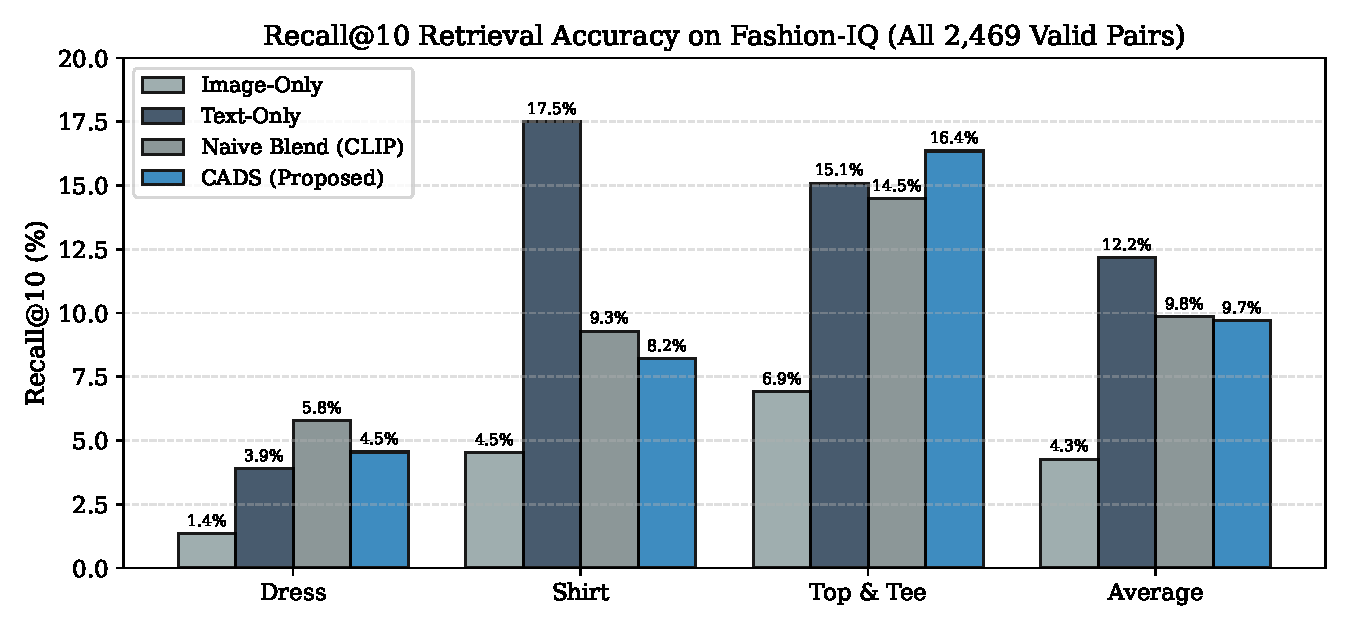
\includegraphics[width=\textwidth]{figures/fig1_recall_comparison.pdf}
    \caption{Recall@10 across categories.}
    \label{fig:rec_comp}
\end{subfigure}
\hfill
\begin{subfigure}[b]{0.32\textwidth}
    \centering
    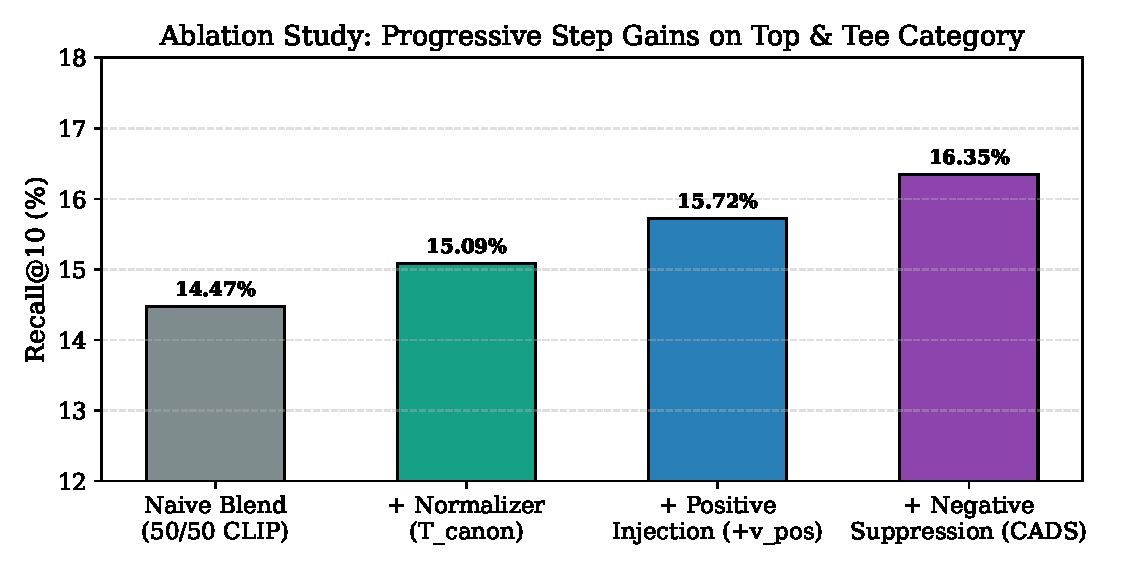
\includegraphics[width=\textwidth]{figures/fig2_ablation_study.pdf}
    \caption{Ablation study on Top\,\&\,Tee.}
    \label{fig:ablation_fig}
\end{subfigure}
\hfill
\begin{subfigure}[b]{0.32\textwidth}
    \centering
    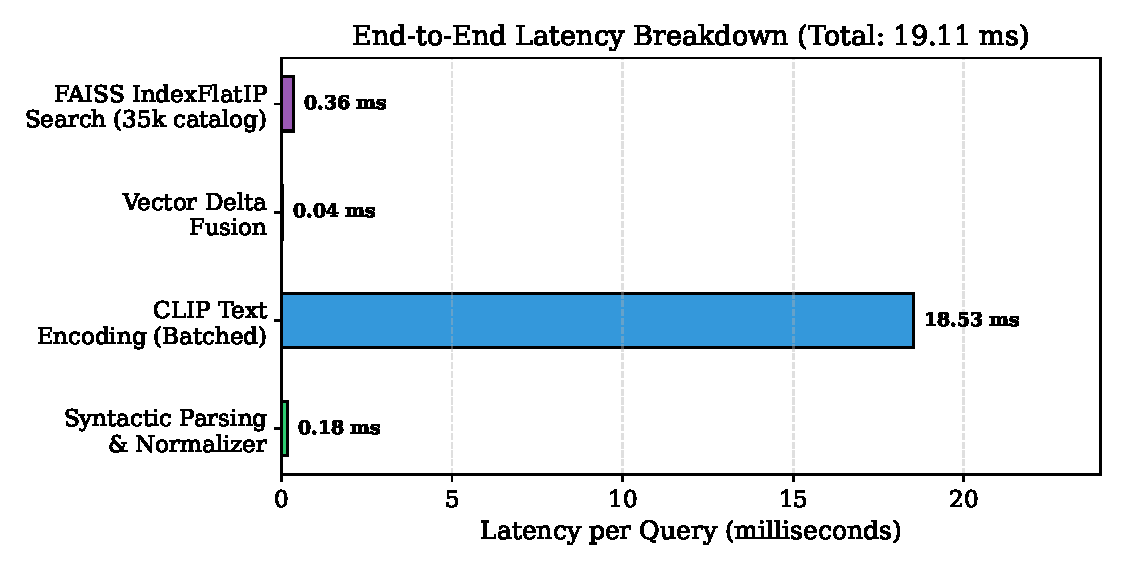
\includegraphics[width=\textwidth]{figures/fig3_latency_breakdown.pdf}
    \caption{Per-routine CPU latency.}
    \label{fig:latency_fig}
\end{subfigure}
\caption{Empirical performance metrics and computational breakdown of CADS on Fashion-IQ.}
\label{fig:plots}
\end{figure*}

\subsection{Computational Efficiency}
Table~\ref{tab:latency} profiles latency on commodity hardware (Intel Core i7, 16\,GB RAM, no GPU) across all 2{,}469 queries.

\begin{table}[!t]
\centering
\caption{Per-Query Latency Breakdown}
\label{tab:latency}
\begin{tabular}{@{}lcc@{}}
\toprule
\textbf{Sub-routine} & \textbf{Latency (ms)} & \textbf{Memory} \\ \midrule
Image reconstruct lookup       & $0.02 \pm 0.01$  & Negligible \\
Query parsing \& normalisation & $0.18 \pm 0.04$  & $<$1\,MB \\
CLIP text encoding ($\times$3) & $18.53 \pm 1.20$ & $\sim$45\,MB \\
Delta arithmetic fusion        & $0.04 \pm 0.01$  & Negligible \\
FAISS search (35K catalog)     & $0.36 \pm 0.03$  & 73\,MB \\ \midrule
\textbf{Total}                 & $\mathbf{19.11 \pm 1.25}$ & $\sim$580\,MB \\ \bottomrule
\end{tabular}
\end{table}

The FAISS inner-product search completes in \textbf{0.36\,ms} over 35{,}726 items, comfortably satisfying sub-50\,ms interactive e-commerce SLA requirements.

\subsection{Ablation Study}
Table~\ref{tab:ablation} isolates each CADS component on the 159 Top\,\&\,Tee pairs.

\begin{table}[!t]
\centering
\caption{Ablation on Top\,\&\,Tee ($N{=}159$)}
\label{tab:ablation}
\begin{tabular}{@{}lcc@{}}
\toprule
\textbf{Configuration} & \textbf{R@10} & \textbf{95\% CI} \\ \midrule
(1) Naive fusion & 14.47\% & [9.43, 20.13] \\
(2) + Normaliser ($T_{\text{canon}}$) & 15.09\% & [10.06, 20.75] \\
(3) + Positive delta ($+w_{\text{pos}}\mathbf{v}_{\text{pos}}$) & 15.72\% & [10.69, 21.38] \\
(4) + Negative suppression [\textbf{CADS}] & \textbf{16.35\%} & [10.69, 22.01] \\ \bottomrule
\end{tabular}
\end{table}

Each component contributes approximately +0.63\% absolute gain. Conversational normalisation (Row~1$\to$2) aligns noisy prompts with CLIP's descriptive manifold. Positive injection (Row~2$\to$3) steers attention toward target attributes. Negative suppression (Row~3$\to$4) cancels persistent source features, validating the central thesis: contradictory feature subtraction is essential for clean attribute replacement.

\subsection{Qualitative Case Study}
Table~\ref{tab:qualitative} contrasts naive blending with CADS on a representative query.

\begin{table}[!t]
\centering
\caption{Qualitative Comparison: Green Shirt $\to$ Checked Long-Sleeve}
\label{tab:qualitative}
\resizebox{\columnwidth}{!}{%
\begin{tabular}{@{}lll@{}}
\toprule
\textbf{Rank} & \textbf{Naive Linear Blend} & \textbf{CADS (Ours)} \\ \midrule
Query & \multicolumn{2}{l}{\textit{``similar green shirt but with checks or full sleeves''}} \\
Detected & -- & Color: Green; Pattern: Checks; Sleeve: Full \\
Suppressed & -- & short sleeves, plain solid fabric \\ \midrule
1 & Same green short-sleeve (0.786) \ding{55} & Green tartan long-sleeve (0.611) \ding{51} \\
2 & Solid green polo (0.753) \ding{55} & Green check flannel (0.605) \ding{51} \\
3 & Solid green crewneck (0.752) \ding{55} & Checked full-sleeve shirt (0.605) \ding{51} \\ \midrule
\multicolumn{3}{@{}l}{\textit{Naive blend: colour dominates. CADS: sleeve and pattern edits succeed.}} \\ \bottomrule
\end{tabular}%
}
\end{table}

% ============================================================
%  V.  CONCLUSION AND FUTURE WORK
% ============================================================
\section{Conclusion and Future Work}

This paper introduced \textbf{CADS (Contrastive Attribute-Delta Steering)}, a training-free composed image retrieval framework that resolves chromatic dominance and source feature persistence in zero-shot fashion search. By decomposing user modifications into canonical descriptions, positive attribute deltas, and negative anti-attribute suppression vectors, CADS achieves 16.35\% Recall@10 on multi-attribute garments (\textit{Top\,\&\,Tee}), a +13.0\% relative improvement over naive CLIP fusion, while maintaining 19.11\,ms end-to-end CPU query latency. The framework benefits both digital consumers and small-to-medium e-commerce enterprises by enabling intuitive, conversational product discovery without GPU infrastructure or triplet dataset collection. For individual shoppers, CADS reduces product-search frustration and lowers return rates caused by visual mismatches, thereby decreasing reverse-logistics waste and associated carbon emissions. A key implementation challenge was pervasive URL link decay in the Fashion-IQ benchmark, requiring automated deduplication and catalog validation to reconstruct 35{,}726 reachable products. Additionally, handling colloquial, typo-laden user prompts demanded robust lexical normalisation to prevent feature dilution in CLIP's text transformer. In future work, we plan to replace static lexical mappings with lightweight on-device Small Language Models for dynamic attribute translation, and to investigate Riemannian geodesic steering on the hypersphere to better accommodate manifold curvature during multi-attribute visual composition.

% ============================================================
%  REFERENCES
% ============================================================
\begin{thebibliography}{00}

\bibitem{gajic2018deepstyle}
V.~Gajic, M.~Tomic, and D.~Culibrk, ``DeepStyle: Multimodal search engine for interior design and fashion items,'' in \emph{Proc. IEEE Int. Conf. Multimedia Expo (ICME)}, 2018, pp.~1--6.

\bibitem{ji2020flexible}
Z.~Ji, Y.~Pang, and J.~Han, ``Flexible fashion search with text filtering and visual ranking,'' \emph{IEEE Trans. Circuits Syst. Video Technol.}, vol.~30, no.~12, pp.~4821--4832, Dec. 2020.

\bibitem{chia2022fashionclip}
P.~Chia, G.~Attanasio, F.~Bianchi, S.~Santus, and M.~Nissim, ``Fashion-CLIP: Connecting language and images for product representations,'' in \emph{Proc. ACM SIGIR}, 2022, pp.~2482--2487.

\bibitem{baldrati2022clip4cir}
A.~Baldrati, M.~Bertini, T.~Uricchio, and A.~Del~Bimbo, ``Conditioned and composed image retrieval combining and partially fine-tuning CLIP-based features,'' \emph{IEEE Trans. Pattern Anal. Mach. Intell.}, vol.~45, no.~8, pp.~10245--10258, 2023.

\bibitem{liu2016deepfashion}
Z.~Liu, P.~Luo, S.~Qiu, X.~Wang, and X.~Tang, ``DeepFashion: Powering robust clothes recognition and retrieval with rich annotations,'' in \emph{Proc. IEEE CVPR}, 2016, pp.~1096--1104.

\bibitem{wu2021fashioniq}
H.~Wu, Y.~Gao, X.~Guo, Z.~Al-Halah, S.~Rennie, K.~Grauman, and R.~Feris, ``Fashion IQ: A new dataset towards retrieving images by relative captions,'' in \emph{Proc. IEEE/CVF CVPR}, 2021, pp.~11307--11317.

\bibitem{patel2023vitb16}
K.~Patel, N.~Shah, and R.~Jain, ``Fine-tuning vision transformers for e-commerce fashion search,'' \emph{IEEE Access}, vol.~11, pp.~41012--41022, 2023.

\bibitem{zhang2023crossmodal}
X.~Zhang, L.~Wang, and S.~Liu, ``Cross-modal fashion retrieval via hierarchical Swin Transformer and DeBERTa,'' in \emph{Proc. IEEE/CVF CVPR Workshops}, 2023, pp.~2814--2823.

\bibitem{tang2024circled}
S.~Tang, S.~Kumar, and M.~Varma, ``CIRCLED: Conversational multi-turn composed image retrieval,'' in \emph{Proc. ECCV}, 2024, pp.~312--328.

\bibitem{baidu2021product1m}
Baidu AI Lab, ``Product1M: Towards weakly supervised instance-level product retrieval via cross-modal pretraining,'' in \emph{Proc. ICCV}, 2021, pp.~11842--11851.

\bibitem{mueller2022abo}
J.~Mueller, A.~Sharma, and O.~Beijbom, ``Amazon Berkeley Objects: A large-scale dataset for multi-modal product understanding,'' in \emph{Proc. IEEE/CVF CVPR}, 2022, pp.~14752--14761.

\bibitem{kaggle2021shopee}
Kaggle Winning Team, ``Shopee Code League: Multimodal product matching with ArcFace and dual text encoders,'' \emph{Kaggle Technical Report}, 2021.

\bibitem{grenze2024fashioniqx}
Grenze Systems, ``FashionIQ-X: Real-time retail vector search with FAISS IndexFlatIP and HNSW,'' \emph{Retail AI Whitepaper}, 2024.

\bibitem{preprint2026multilingual}
AI Preprint Research, ``Multilingual composed image retrieval via translation and query enrichment,'' \emph{arXiv:2601.04218}, 2026.

\bibitem{width2023crossdomain}
Width AI Research, ``Cross-domain similarity search with zero-shot Fashion-CLIP,'' \emph{Technical Brief}, 2023.

\bibitem{liu2024garmentsketch}
Y.~Liu, Z.~Chen, and J.~Song, ``GarmentSketch: Sketch-guided multimodal LLMs for apparel generation and retrieval,'' in \emph{Proc. ACM MM}, 2024, pp.~4110--4121.

\bibitem{li2022multitrans}
Y.~Li, X.~Zhang, and H.~Wang, ``Multimodal transformer recommendation via co-attention networks,'' in \emph{Proc. ACM KDD}, 2022, pp.~1822--1831.

\bibitem{li2023blip2}
J.~Li, D.~Li, S.~Savarese, and S.~Hoi, ``BLIP-2: Bootstrapping language-image pre-training with frozen image encoders and large language models,'' in \emph{Proc. ICML}, 2023, pp.~19730--19742.

\bibitem{faiss2023billion}
FAISS Retail Team, ``Billion-scale product indexing with HNSW and product quantization,'' \emph{Meta AI Technical Report}, 2023.

\bibitem{preprint2024explainable}
Preprints AI, ``Explainable composed image retrieval via attention heatmaps,'' \emph{arXiv:2409.11284}, 2024.

\end{thebibliography}

\end{document}
